\section{Introducción}

\subsection{Diagrama de Diseño}

\begin{figure}[H]
    \centering
     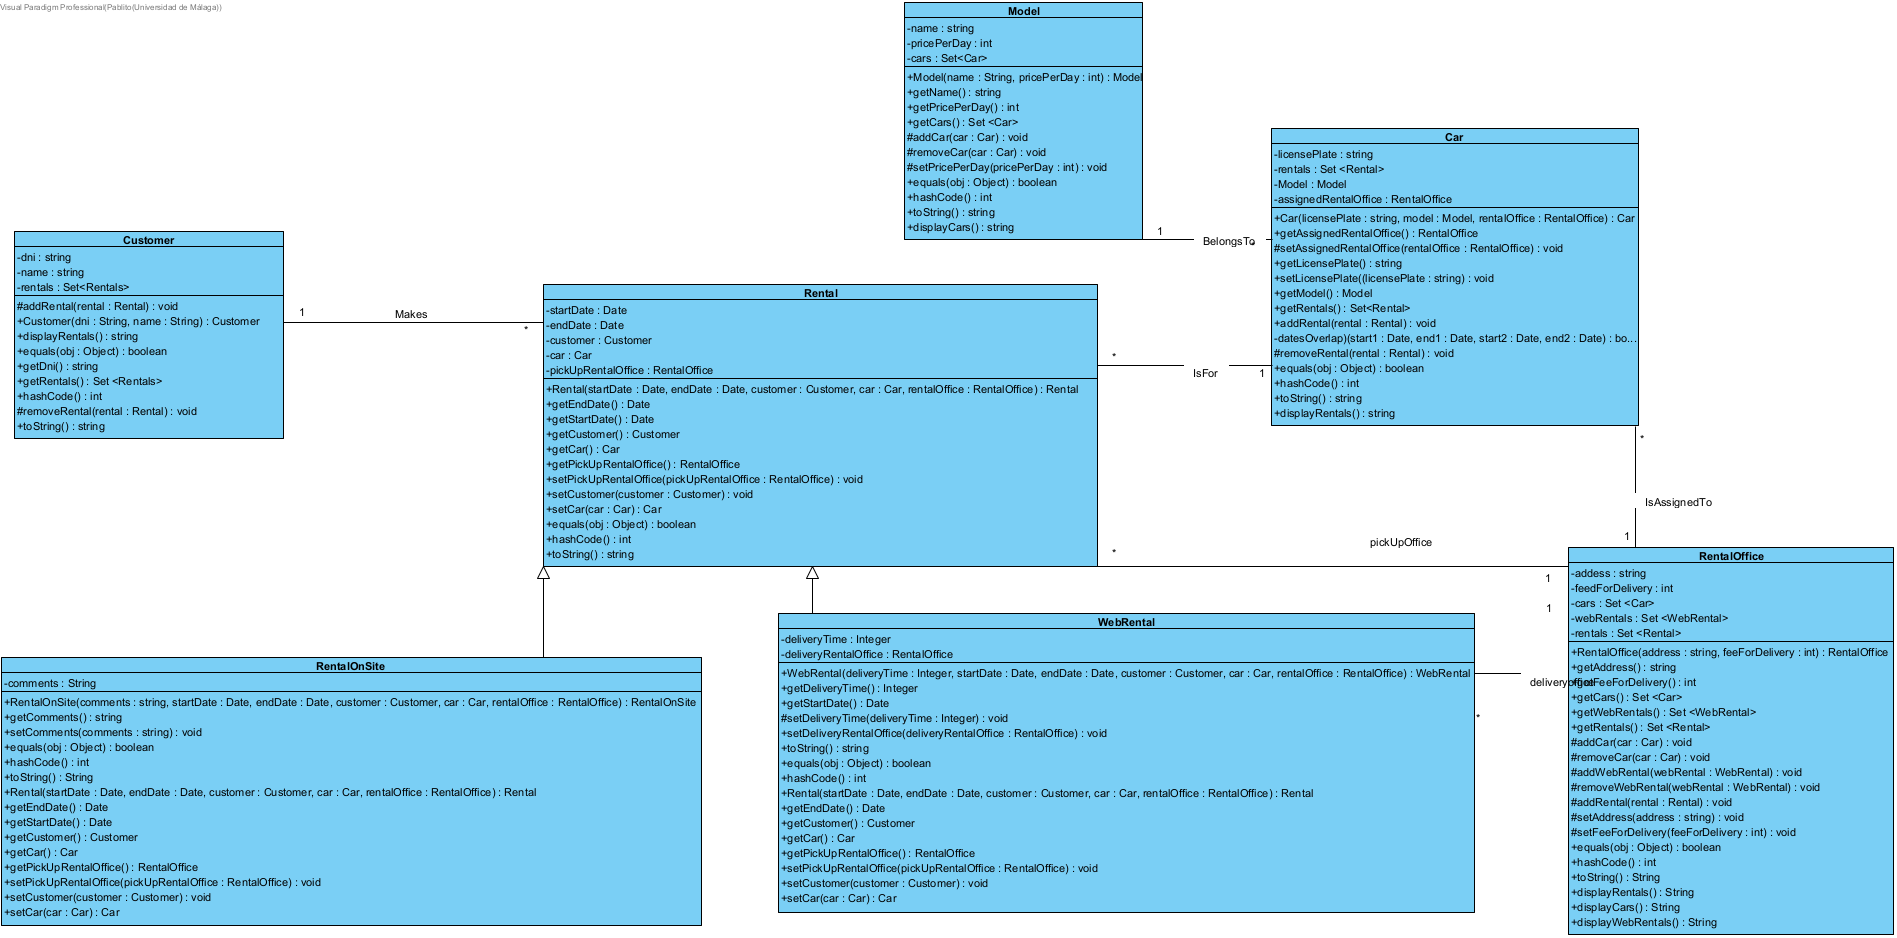
\includegraphics[width=1\linewidth]{assets/diagramas/UML_Esqueleto.png}
     \caption{Diagrama de Diseño del esqueleto}
\end{figure}

\subsection{Cambios respecto a la implementación original}

\subsubsection{Model}

\subsubsection*{Atributos}

\begin{itemize}
    \item \textbf{name: String}: Nombre del modelo. Este valor es inmutable.
    \item \textbf{pricePerDay: int}: Precio por día asociado al modelo.
    \item \textbf{cars: Set$<$Car$>$}: Conjunto de coches asociados al modelo de Coche. Este conjunto es  inmutable.
\end{itemize}

\subsubsection*{Operaciones}

\begin{itemize}
    \item \textbf{Model(name : String, pricePerDay : int) : Model}: 
    Constructor que inicializa un modelo con su nombre y precio por día. Garantiza que el nombre no sea \texttt{null} y que el precio por día sea positivo.

    \item \textbf{getName() : String}: Devuelve el nombre del modelo.
    \item \textbf{getPricePerDay() : int}: Devuelve el precio por día del modelo.
    \item \textbf{getCars() : Set<Car>}: Devuelve el conjunto de coches asociados al modelo.
    \item \textbf{addCar(car : Car) : void}: Añade un coche al conjunto de coches del modelo. 
    \item \textbf{removeCar(car : Car) : void}: Elimina un coche del conjunto de coches del modelo.
    \item \textbf{setPricePerDay(pricePerDay : int) : void}: Actualiza el precio por día del modelo.
    \item \textbf{equals(obj : Object) : boolean}: Compara dos modelos para determinar si son iguales basándose en su nombre.
    \item \textbf{hashCode() : int}: Genera un código hash basado en el nombre del modelo.
    \item \textbf{toString() : String}: Devuelve un string con el nombre del modelo, su precio por día y el conjunto de coches.
    \item \textbf{displayCars() : String}: Devuelve los detalles de todos los coches del modelo.
\end{itemize}

\subsubsection{Car}

\subsubsection*{Atributos}

\begin{itemize}
    \item \textbf{licensePlate: String}: Matrícula del coche.
    \item \textbf{rentals: Set$<$Rental$>$}: Conjunto de alquileres asociados al coche. Este conjunto es inmutable.
    \item \textbf{model: Model}: Modelo del coche. Este valor es inmutable.
    \item \textbf{assignedRentalOffice: RentalOffice}: Oficina de alquiler asignada al coche.
\end{itemize}

\subsubsection*{Operaciones}

\begin{itemize}
    \item \textbf{Car(licensePlate : String, model : Model, rentalOffice : RentalOffice) : Car}: 
    Constructor que inicializa un coche con su matrícula, modelo y oficina de alquiler asignada.
    \item \textbf{getAssignedRentalOffice() : RentalOffice}: Devuelve la oficina de alquiler asignada al coche.
    \item \textbf{setAssignedRentalOffice(rentalOffice : RentalOffice) : void}: Actualiza la oficina de alquiler asignada al coche.
    \item \textbf{getLicensePlate() : String}: Devuelve la matrícula del coche.
    \item \textbf{setLicensePlate(licensePlate : String) : void}: Actualiza la matrícula del coche.
    \item \textbf{getModel() : Model}: Devuelve el modelo del coche.
    \item \textbf{getRentals() : Set$<$Rental$>$}: Devuelve el conjunto de alquileres del al coche.
    \item \textbf{addRental(rental : Rental) : void}: Añade un alquiler al conjunto de alquileres del coche. 
    \item \textbf{removeRental(rental : Rental) : void}: Elimina un alquiler del conjunto de alquileres del coche.
    \item \textbf{equals(obj : Object) : boolean}: Compara dos coches para determinar si son iguales basándose en su matrícula.
    \item \textbf{hashCode() : int}: Genera un código hash basado en la matrícula del coche.
    \item \textbf{toString() : String}: Devuelve un string  del coche mostrando su matrícula.
    \item \textbf{displayRentals() : String}: Devuelve los detalles de todos los alquileres del coche.
\end{itemize}

\subsubsection*{Validaciones y Consideraciones}

\begin{itemize}
    \item La relación entre un coche y su oficina de alquiler es bidireccional. Si se actualiza la oficina, también se actualiza en la oficina anterior y la nueva.
    \item Se verifica que las fechas de un nuevo alquiler no se solapen con las de los alquileres existentes, garantizando la coherencia.
    \item El conjunto \texttt{rentals} se expone como una colección inmutable para evitar modificaciones desde el exterior.
\end{itemize}


\subsubsection{Customer}

\subsubsection*{Atributos}

\begin{itemize}
    \item \textbf{dni: String}: Es el DNI del cliente, un identificador único. No se permite modificarlo después de inicializarlo.
    \item \textbf{name: String}: Es el nombre del cliente. No se permite modificarlo después de inicializarlo.
    \item \textbf{rentals: Set$<$Rental$>$}: Conjunto de todos los alquileres de cliente.
\end{itemize}

\subsubsection*{Operaciones}

\begin{itemize}
    \item \textbf{Customer(dni : String, name : String) : Customer}: Constructor que inicializa un cliente con un DNI y un nombre.
    \item \textbf{getDni() : String}: Devuelve el DNI del cliente.
    \item \textbf{getName() : String}: Devuelve el nombre del cliente.
    \item \textbf{getRentals() : Set$<$Rental$>$}: Devuelve el conjunto de alquileres asociados al cliente.
    \item \textbf{addRental(rental : Rental) : void}: Agrega un alquiler al conjunto de alquileres del cliente.
    \item \textbf{removeRental(rental : Rental) : void}: Elimina un alquiler del conjunto de alquileres del cliente.
    \item \textbf{equals(obj : Object) : boolean}: Compara dos clientes por DNI para determinar si son iguales.
    \item \textbf{hashCode() : int}: Genera un código hash basado en el DNI del cliente.
    \item \textbf{toString() : String}: Devuelve un string con el dni, nombre y lista de alquileres de un cliente.
    \item \textbf{displayRentals() : String}: Devuelve los detalles de todos los alquileres del cliente.
\end{itemize}


\subsubsection{Rental}

\subsubsection*{Atributos}

\begin{itemize}
    \item \textbf{startDate: Date}: Fecha del inicio del alquiler. Este valor es inmutable.
    \item \textbf{endDate: Date}: Fecha de la finalización del alquiler. Este valor es inmutable.
    \item \textbf{customer: Customer}: Cliente asociado al alquiler. 
    \item \textbf{car: Car}: Coche asociado al alquiler. 
    \item \textbf{pickUpRentalOffice: RentalOffice}: Oficina de recogida del coche.
\end{itemize}

\subsubsection*{Operaciones}

\begin{itemize}
    \item \textbf{Rental(startDate : Date, endDate : Date, customer : Customer, car : Car, rentalOffice : RentalOffice) : Rental}: 
    Constructor que inicializa un alquiler con las fechas de inicio y fin, cliente, coche y oficina de recogida.
    
    \item \textbf{getStartDate() : Date}: Devuelve la fecha de inicio del alquiler.
    \item \textbf{getEndDate() : Date}: Devuelve la fecha de finalización del alquiler.
    \item \textbf{getCustomer() : Customer}: Devuelve el cliente asociado al alquiler.
    \item \textbf{getCar() : Car}: Devuelve el coche asociado al alquiler.
    \item \textbf{getPickUpRentalOffice() : RentalOffice}: Devuelve la oficina de recogida del coche.
    \item \textbf{setPickUpRentalOffice(rentalOffice : RentalOffice) : void}: Actualiza la oficina de recogida del coche.
    \item \textbf{setCustomer(customer : Customer) : void}: Actualiza el cliente asociado al alquiler.
    \item \textbf{setCar(car : Car) : void}: Actualiza el coche asociado al alquiler.
    \item \textbf{equals(o : Object) : boolean}: Compara dos alquileres para ver si son iguales mediante las fechas de inicio y fin, el cliente, y el coche.
    \item \textbf{hashCode() : int}: Genera un código hash basado en las fechas de inicio, fin, el cliente y el coche.
    \item \textbf{toString() : String}: Devuelve un string con la clase de alquiler, su fecha de inicio y su fecha de fin.
\end{itemize}

\subsubsection{RentalOnSite}

\subsubsection*{Atributos}

\begin{itemize}
    \item \textbf{comments: String}: Comentarios sobre el alquiler. 
\end{itemize}

\subsubsection*{Operaciones}

\begin{itemize}
    \item \textbf{RentalOnSite(comments : String, startDate : Date, endDate : Date, customer : Customer, car : Car, rentalOffice : RentalOffice) : RentalOnSite}: 
    Constructor que inicializa un alquiler presencial con comentarios opcionales, las fechas de inicio y fin, cliente, coche, y oficina de recogida.

    \item \textbf{RentalOnSite(startDate : Date, endDate : Date, customer : Customer, car : Car, rentalOffice : RentalOffice) : RentalOnSite}: 
    Constructor alternativo que inicializa un alquiler presencial pero sin comentarios.

    \item \textbf{getComments() : String}: Devuelve los comentarios asociados al alquiler.
    \item \textbf{setComments(comments : String) : void}: Actualiza los comentarios asociados al alquiler.
    \item \textbf{equals(o : Object) : boolean}: Compara dos alquileres para determinar si son iguales, mediante los atributos heredados y los comentarios.
    \item \textbf{hashCode() : int}: Genera un código hash basado en los atributos heredados y los comentarios.
    \item \textbf{toString() : String}: Devuelve un string con los atributos heredados y los comentarios.
\end{itemize}

\subsubsection{WebRental}

\subsubsection*{Atributos}

\begin{itemize}
    \item \textbf{deliveryTime: Integer}: Tiempo de entrega del Choche en la Oficina correspondiente. 
    \item \textbf{deliveryRentalOffice: RentalOffice}: Oficina de entrega del alquiler.
\end{itemize}

\subsubsection*{Operaciones}

\begin{itemize}
    \item \textbf{WebRental(deliveryTime : Integer, startDate : Date, endDate : Date, customer : Customer, car : Car, rentalOffice : RentalOffice) : WebRental}: 
    Constructor que inicializa un alquiler web con tiempo de entrega, fechas de inicio y fin, cliente, coche, y oficina de entrega. La oficina de recogida es la misma que la del coche al crear el alquiler.

    \item \textbf{getDeliveryTime() : Integer}: Devuelve el tiempo de entrega asociado al alquiler.
    \item \textbf{setDeliveryTime(deliveryTime : Integer) : void}: Actualiza el tiempo de entrega. 
    \item \textbf{setDeliveryRentalOffice(deliveryRentalOffice : RentalOffice) : void}: Actualiza la oficina de entrega asociada al alquiler.
    \item \textbf{equals(o : Object) : boolean}: Compara dos alquileres para determinar si son iguales, mediante atributos heredados, el tiempo de entrega y la oficina de entrega.
    \item \textbf{hashCode() : int}: Genera un código hash basado en los atributos heredados, el tiempo de entrega y la oficina de entrega.
    \item \textbf{toString() : String}: Devuelve un string con los atributos heredados y el tiempo de entrega.
\end{itemize}

\subsubsection{RentalOffice}

\subsubsection*{Atributos}

\begin{itemize}
    \item \textbf{address: String}: Dirección de la oficina de alquiler. 
    \item \textbf{feeForDelivery: Integer}: Tarifa de entrega de la oficina de alquiler
    \item \textbf{cars: Set$<$Car$>$}: Conjunto de coches disponibles en la oficina de alquiler.
    \item \textbf{webRentals: Set$<$WebRental$>$}: Conjunto de alquileres web asociados a la oficina. 
    \item \textbf{rentals: Set$<$Rental$>$}: Conjunto de alquileres asociados a la oficina.
\end{itemize}

\subsubsection*{Operaciones}

\begin{itemize}
    \item \textbf{RentalOffice(address : String, feeForDelivery : Integer) : RentalOffice}: 
    Constructor que inicializa una oficina de alquiler con una dirección y una tarifa de entrega.
    \item \textbf{getAddress() : String}: Devuelve la dirección de la oficina de alquiler.
    \item \textbf{getFeeForDelivery() : Integer}: Devuelve la tarifa de entrega de la oficina.
    \item \textbf{getCars() : Set$<$Car$>$}: Devuelve el conjunto de coches disponibles en la oficina.
    \item \textbf{getWebRentals() : Set$<$WebRental$>$}: Devuelve el conjunto los alquileres web de la oficina.
    \item \textbf{getRentals() : Set$<$Rental$>$}: Devuelve un conjunto de los alquileres de la oficina.
    \item \textbf{addCar(car : Car) : void}: Añade un coche a la oficina.
    \item \textbf{removeCar(car : Car) : void}: Elimina un coche de la oficina.
    \item \textbf{addWebRental(webRental : WebRental) : void}: Añade un alquiler web a la oficina.
    \item \textbf{removeWebRental(webRental : WebRental) : void}: Elimina un alquiler web de la oficina.
    \item \textbf{addRental(rental : Rental) : void}: Añade un alquiler a la oficina.
    \item \textbf{removeRental(rental : Rental) : void}: Elimina un alquiler de la oficina.
    \item \textbf{setAddress(address : String) : void}: Actualiza la dirección de la oficina
    \item \textbf{setFeeForDelivery(feeForDelivery : Integer) : void}: Actualiza la tarifa de entrega de la oficina
    \item \textbf{equals(o : Object) : boolean}: Compara dos oficinas para ver si son iguales, utilizando la dirección.
    \item \textbf{hashCode() : int}: Genera un código hash basado en la dirección de la oficina.
    \item \textbf{toString() : String}: Devuelve un string mostrando la oficina, la dirección, la tarifa de entrega, los coches, los alquileres y los alquileres web.
    \item \textbf{displayCars() : String}: Devuelve un string de todos los coches disponibles en la oficina.
    \item \textbf{displayWebRentals() : String}: Devuelve un string de todos los alquileres web de la oficina.
    \item \textbf{displayRentals() : String}: Devuelve un string de todos los alquileres de la oficina.
\end{itemize}

